\documentclass[12pt,letterpaper]{article}
\usepackage{amsmath,amsthm,amsfonts,amssymb,amscd}
\usepackage{fullpage}
\usepackage{graphicx}
\usepackage{lastpage}
\usepackage{listings}
\lstset{
	numbers=left,
	numbersep=5pt,
	stepnumber=1,
	tabsize=2,
	showstringspaces=false
}
\usepackage{enumerate}
\usepackage{fancyhdr}
\usepackage{hyperref}
\usepackage{mathrsfs}
\usepackage{cancel}
\usepackage{xcolor}
\usepackage[margin=3cm]{geometry}
\setlength{\parindent}{0.0in}
\setlength{\parskip}{0.05in}

% Edit these as appropriate
\newcommand\course{STA561/CS571}
\newcommand\semester{Fall 2013}     % <-- current semester
\newcommand\hwnum{2}                  % <-- homework number
\newcommand\yourname{Matt Dickenson} % <-- your name
\newcommand\login{mcd31}           % <-- your NetID
\newcommand\hwdate{Due: 23 September, 2013}           % <-- HW due date

\newenvironment{answer}[1]{
  \subsubsection*{Problem #1}
}


\pagestyle{fancyplain}
\headheight 35pt
\lhead{\yourname\ \texttt{\login}\\\course\ --- \semester}
\chead{\textbf{\Large Homework \hwnum}}
\rhead{\hwdate}
\headsep 10pt

\begin{document}

\noindent \emph{Homework Notes:} I did not work with anyone else on this homework or refer to resources other than the course notes, textbook, and course Piazza page.

\begin{answer}{1}

\paragraph{A} Using the normal equation $\hat{\beta}=(X^TX)^{-1}(X^TY)$, we can calculate $\hat{\beta}$ in $\mathcal{R}$ with the following program (after loading the data as \texttt{lindata}):

\lstinputlisting[language=R, caption=R Code for 1A, firstline=13, lastline=25, firstnumber=1]{cs571-hw3.r}

Letting $\beta_i$ correspond to $X_i$ and $\beta_0$ represent the intercept, $\hat{\beta}_0=69.94, \hat{\beta}_1=15.12, \hat{\beta}_2=0.32$. 


\paragraph{B}  We can also estimate $\beta$ using online stochastic gradient descent with $\mathcal{R}$'s \texttt{optim} function for minimization:

\lstinputlisting[language=R, caption=R Code for 1B, firstline=28, lastline=42, firstnumber=last]{cs571-hw3.r}

Using this method we reach the same results as above: $\hat{\beta}_0=69.94, \hat{\beta}_1=15.12, \hat{\beta}_2=0.32$. 

\paragraph{C} A third method we can use to estimate $\beta$ is ridge regression, using the following $\mathcal{R}$ code:

\lstinputlisting[language=R, caption=R Code for 1C, firstline=45, lastline=56, firstnumber=last]{cs571-hw3.r}

From this approach we get the estimates $\hat{\beta}_1=3.00, \hat{\beta}_2=0.78$. 

\paragraph{D} Table \ref{rss.train} presents the residual sum of squares (RSS) for the training data using each of the methods above.


\begin{table}[h!]
\caption{Training set RSS for linear regression methods}
\label{rss.train}
\begin{center}
\begin{tabular}{lr}
Method & RSS \\
\hline
Normal equations & 98,729.3 \\
Online stochastic gradient descent & 98,729.3 \\
Ridge regression & 99,005.9
\end{tabular}
\end{center}
\end{table}

% RSS(\beta) = \sum_{i=1}^n (y_i - \beta^T x_i)^2

\paragraph{E} Table \ref{rss.test} presents the residual sum of squares (RSS) for the test data using each of the methods above.

\begin{table}[h!]
\caption{Test set RSS for linear regression methods}
\label{rss.test}
\begin{center}
\begin{tabular}{lr}
Method & RSS \\
\hline
Normal equations & 11,573.2 \\
Online stochastic gradient descent & 11,573.2 \\
Ridge regression & 11,523.5
\end{tabular}
\end{center}
\end{table}

\paragraph{F}

We can now take the predicted blood pressure for a hypothetical female weighing 135 pounds for the three different methods (Table \ref{pred}):

\begin{table}[h!]
\caption{Predicted values}
\label{pred}
\begin{center}
\begin{tabular}{lr}
Method & $\mathbb{E}[Y|X=[1,135]^T,\hat{\beta}]$ \\
\hline
Normal equations & 128.4 \\
Online stochastic gradient descent & 128.4 \\
Ridge regression & 127.2
\end{tabular}
\end{center}
\end{table}

\paragraph{G} Bivariate plots are given in Figures \ref{p1x1} and \ref{p1x2} below, along with regression lines for the three methods used above. The $y$-axis values are $Y-\hat{\beta}_i X_i - \hat{\beta}_0$ and the $x$-axis values are $X_j, j \neq i$. (Note that indices in the $y$-axis label do not correspond to the $X$ and $\hat{\beta}$ subscripts because $\mathcal{R}$ uses 1-based indexing.) Regression lines in the plots for $X_i$ use $\hat{\beta}_i X_i$

\begin{figure}[h!]
\begin{center}
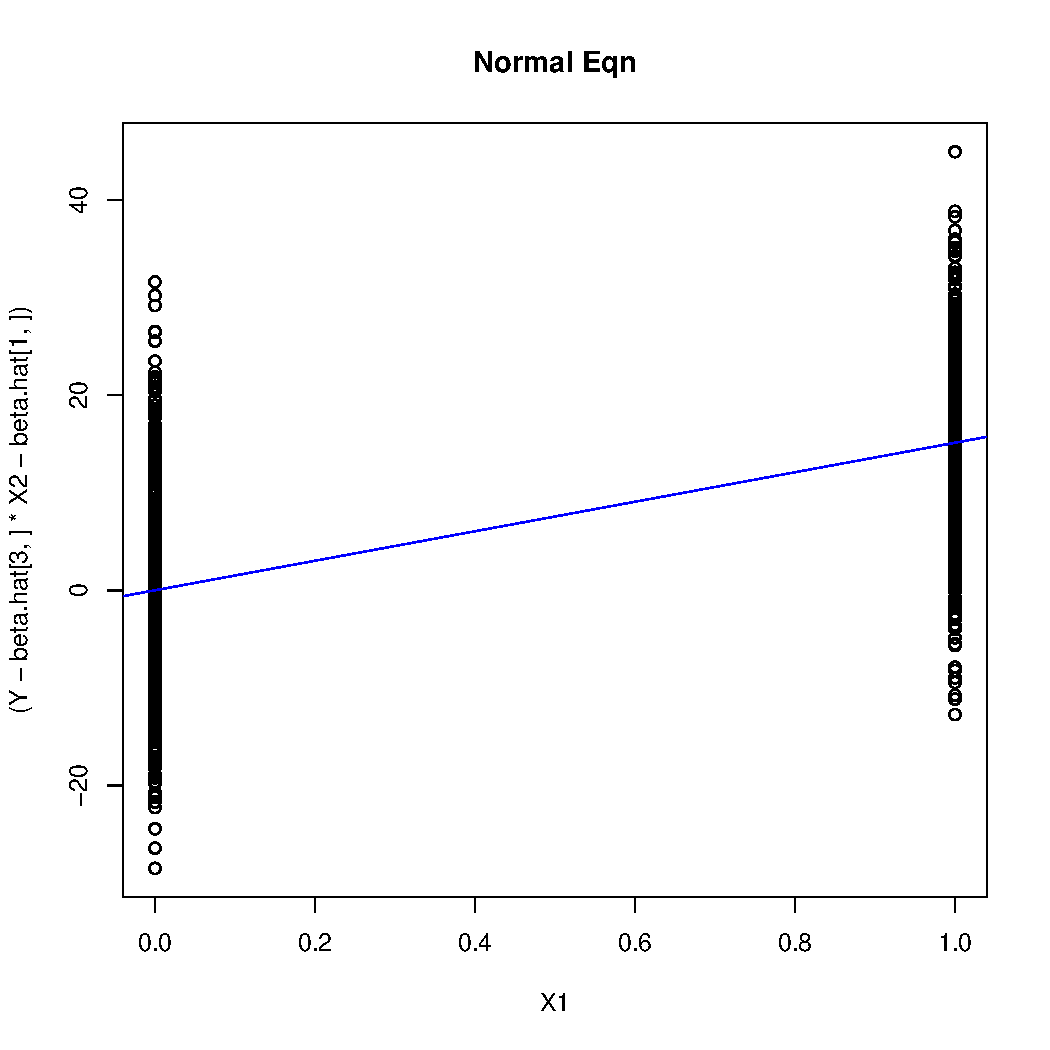
\includegraphics[scale=0.4]{p1x1-normal.pdf}
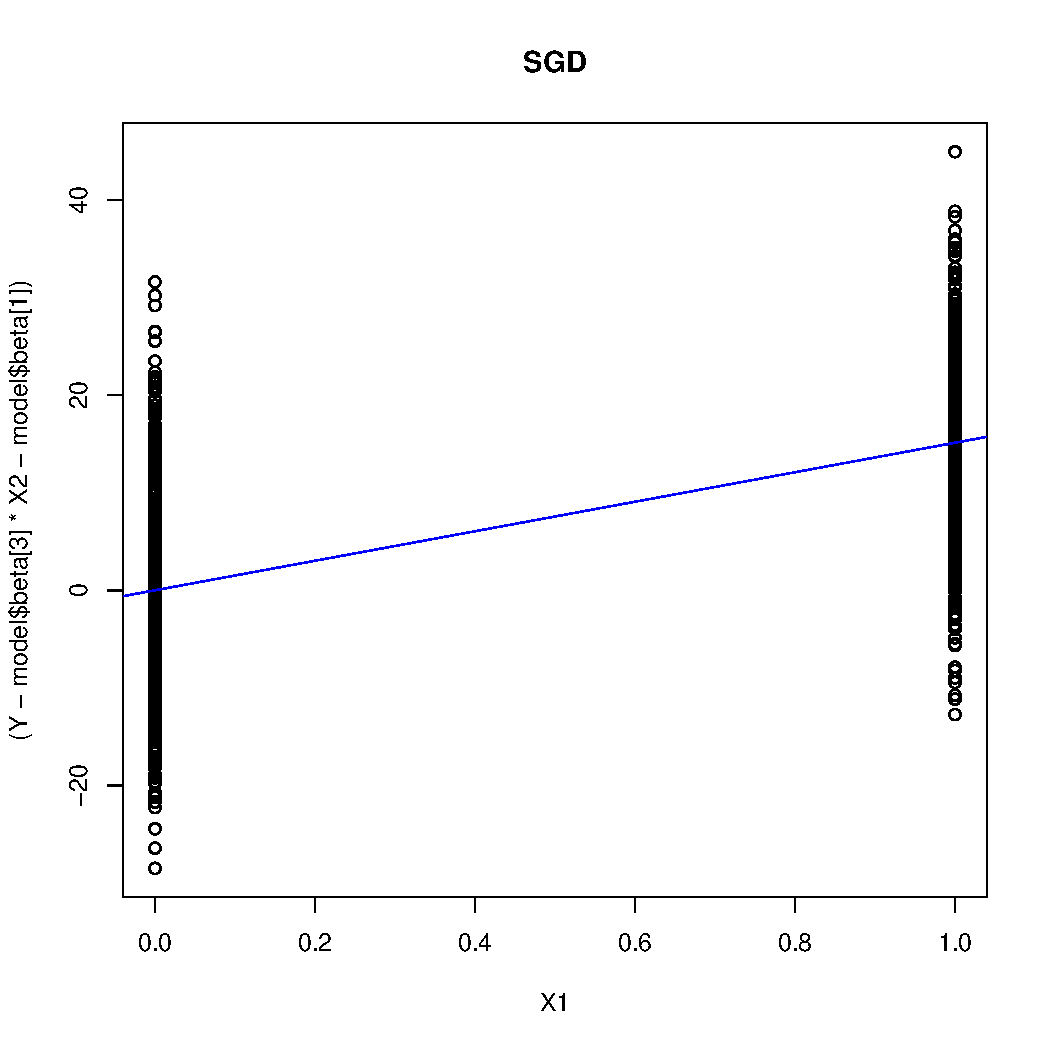
\includegraphics[scale=0.4]{p1x1-sgd.pdf}
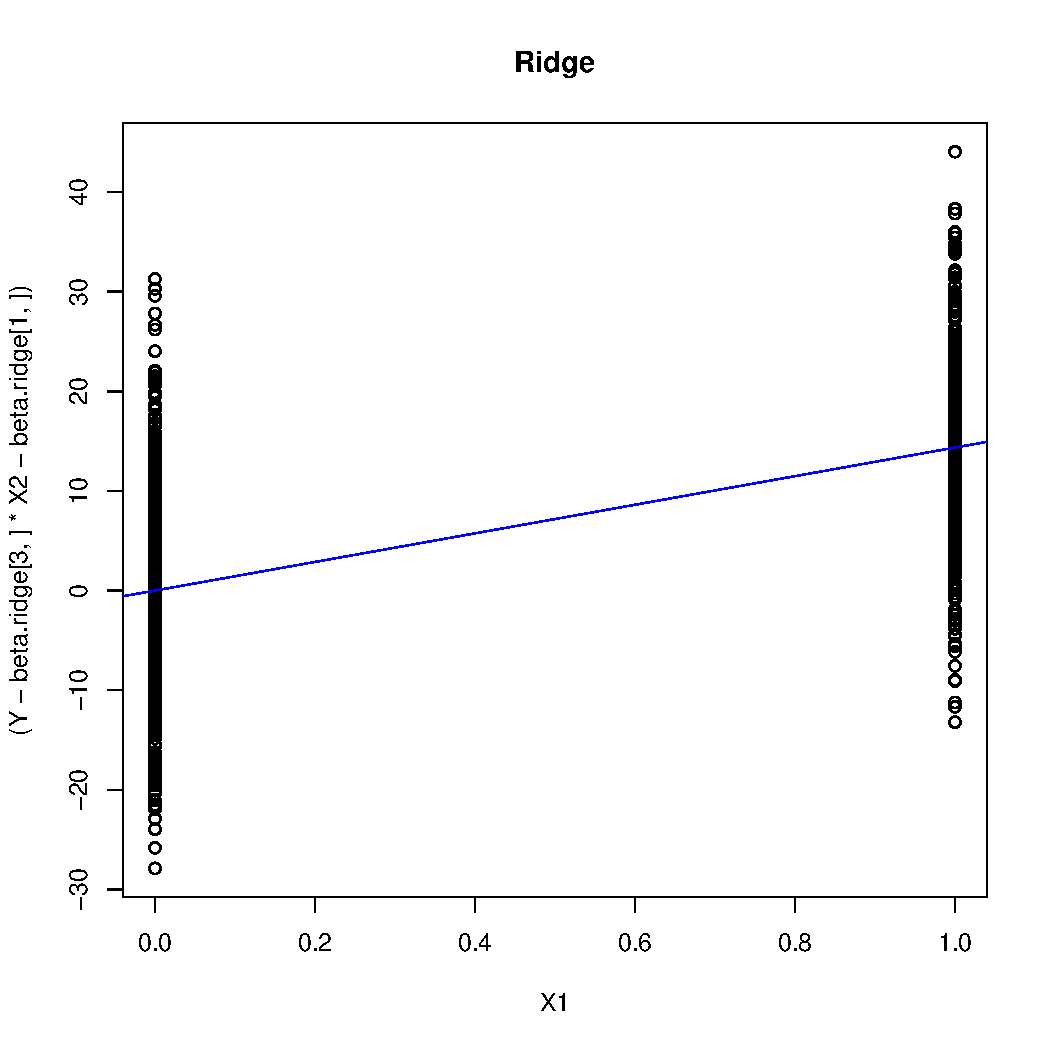
\includegraphics[scale=0.4]{p1x1-ridge.pdf}
\caption{$X_1$ and $Y$ with Regression Lines}
\label{p1x1}
\end{center}
\end{figure}

\begin{figure}[h!]
\begin{center}
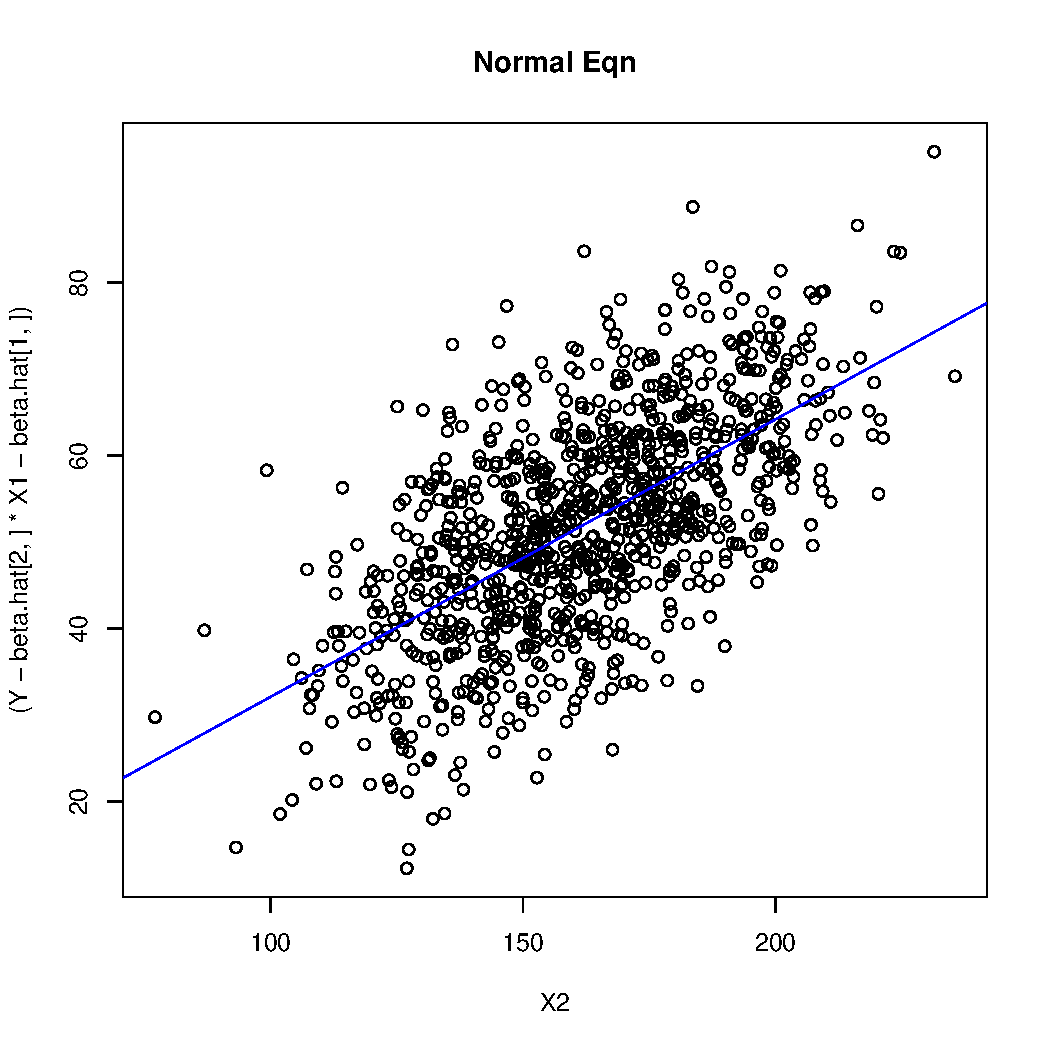
\includegraphics[scale=0.4]{p1x2-normal.pdf}
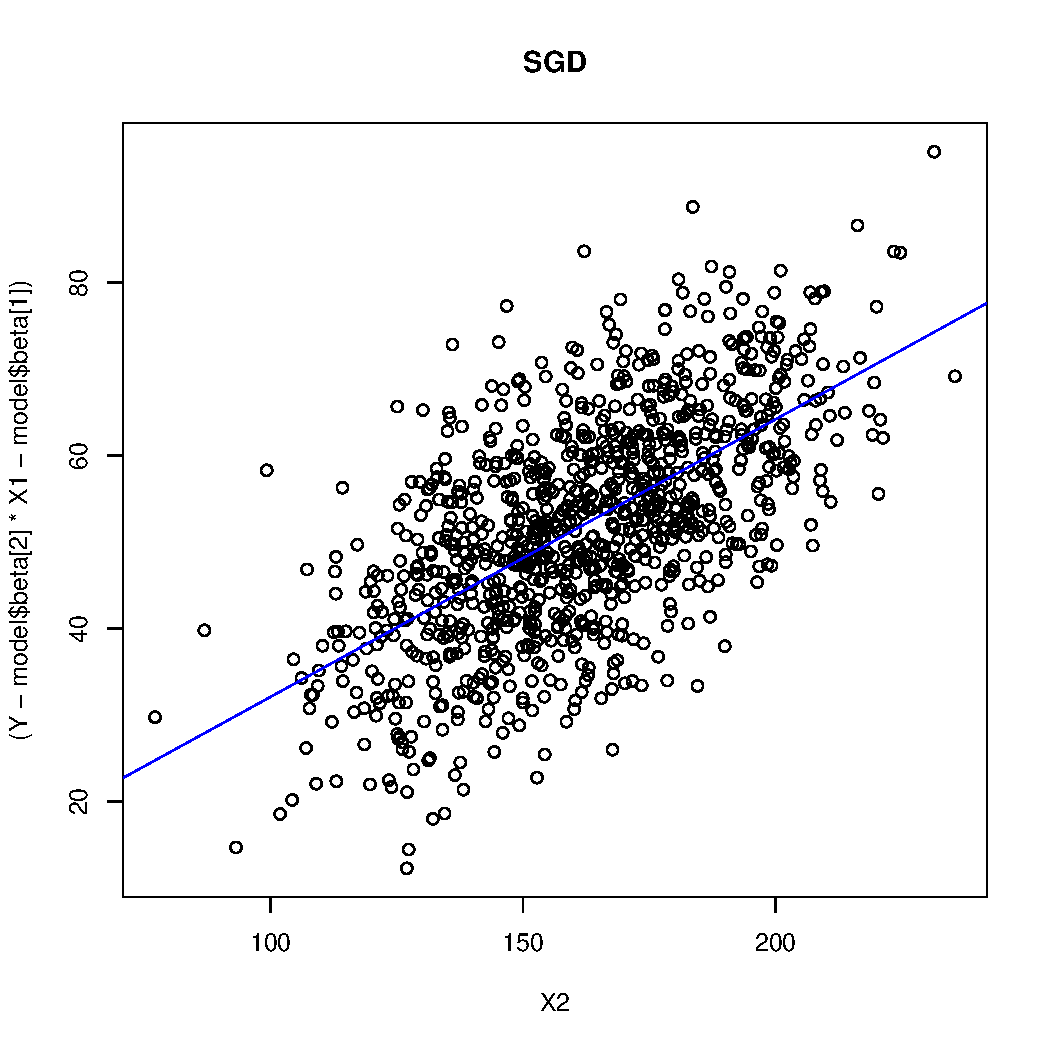
\includegraphics[scale=0.4]{p1x2-sgd.pdf}
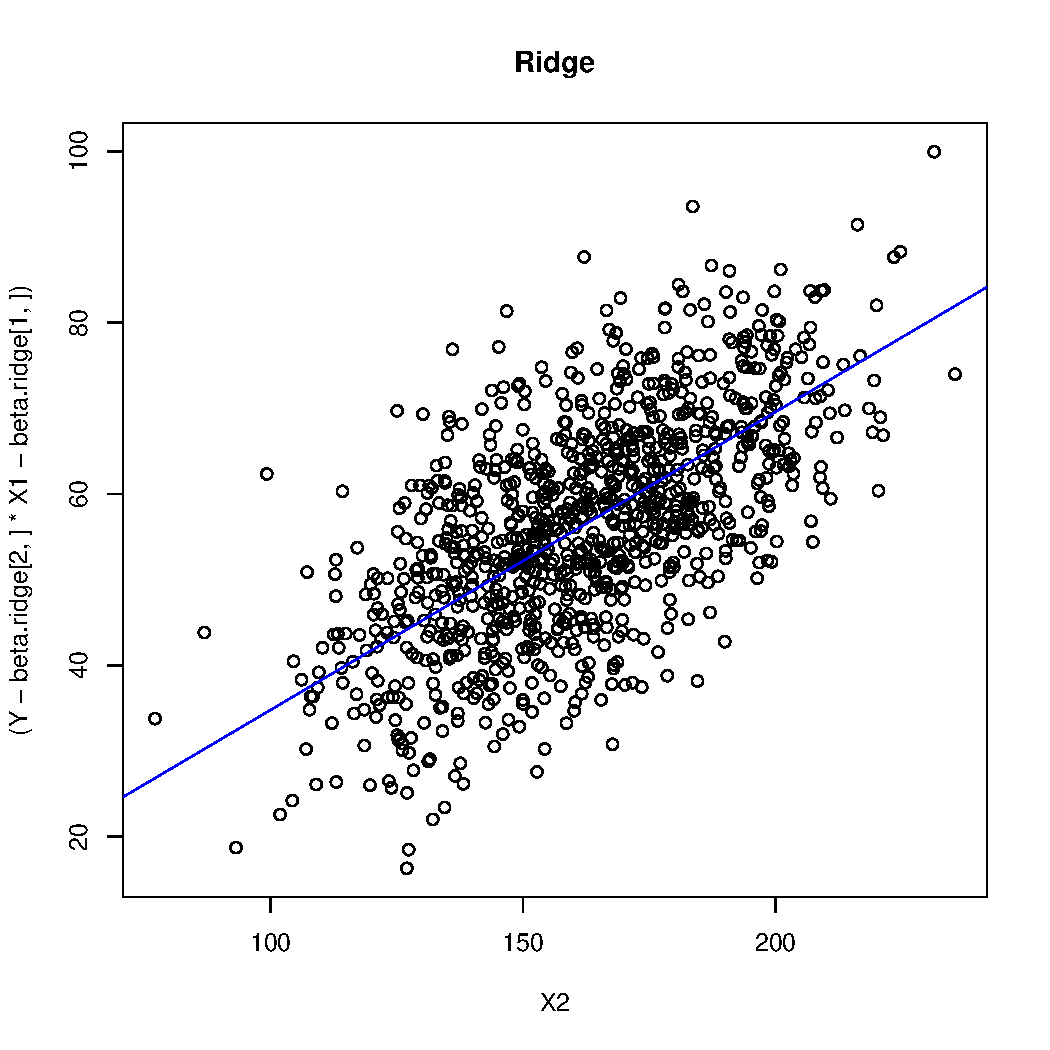
\includegraphics[scale=0.4]{p1x2-ridge.pdf}\caption{$X_2$ and $Y$ with Regression Lines}
\label{p1x2}
\end{center}
\end{figure}

\paragraph{H} Of the three methods used above, ridge regression is the least likely to overfit the data. This is because the $\lambda$ term (using the notation in the MLAPP textbook) helps to regularize the coefficients. This leads to higher RSS in the training data but also makes the coefficients less susceptible to outliers, as evidenced by the lower RSS using the test set data. The other two methods provide no such protection against outliers, and are thus more likely to overfit the training data. 

\paragraph{I} The researchers should use the ridge regresion results. One reason for this is its robustness (relative to the other two methods) to overfitting. This is especially pertinent given the small $n$ of the training data. However, the similarity in the coefficients should help allay any concerns the researchers may have over the differences in the three methods. 

\end{answer}



\newpage
\begin{answer}{2} 

\paragraph{A} The following $\mathcal{R}$ code implements the IRLS algorithm as presented in the MLAPP textbook (after loading the data):

\lstinputlisting[language=R, caption=R Code for 2A, firstline=168, lastline=222, firstnumber=1]{cs571-hw3.r}

\paragraph{B} The RSS($\hat{\beta}$) for the training data is 141.47. 

\paragraph{C} The RSS($\hat{\beta}$) for the test data is 15.73.

\paragraph{F} (\emph{sic}) $\mathbb{E}[Z|X=[1,135]^T,\hat{\beta}] = 0.088$

\paragraph{G} Figures \ref{p2x1} and \ref{p2x2} below plot $X_1$ and $X_2$ with $Z$ and the respective regression line. Because $X_1$ and $Z$ are binary variables, a small random jitter is added to make the points more apparent. 

\begin{figure}[h!]
\begin{center}
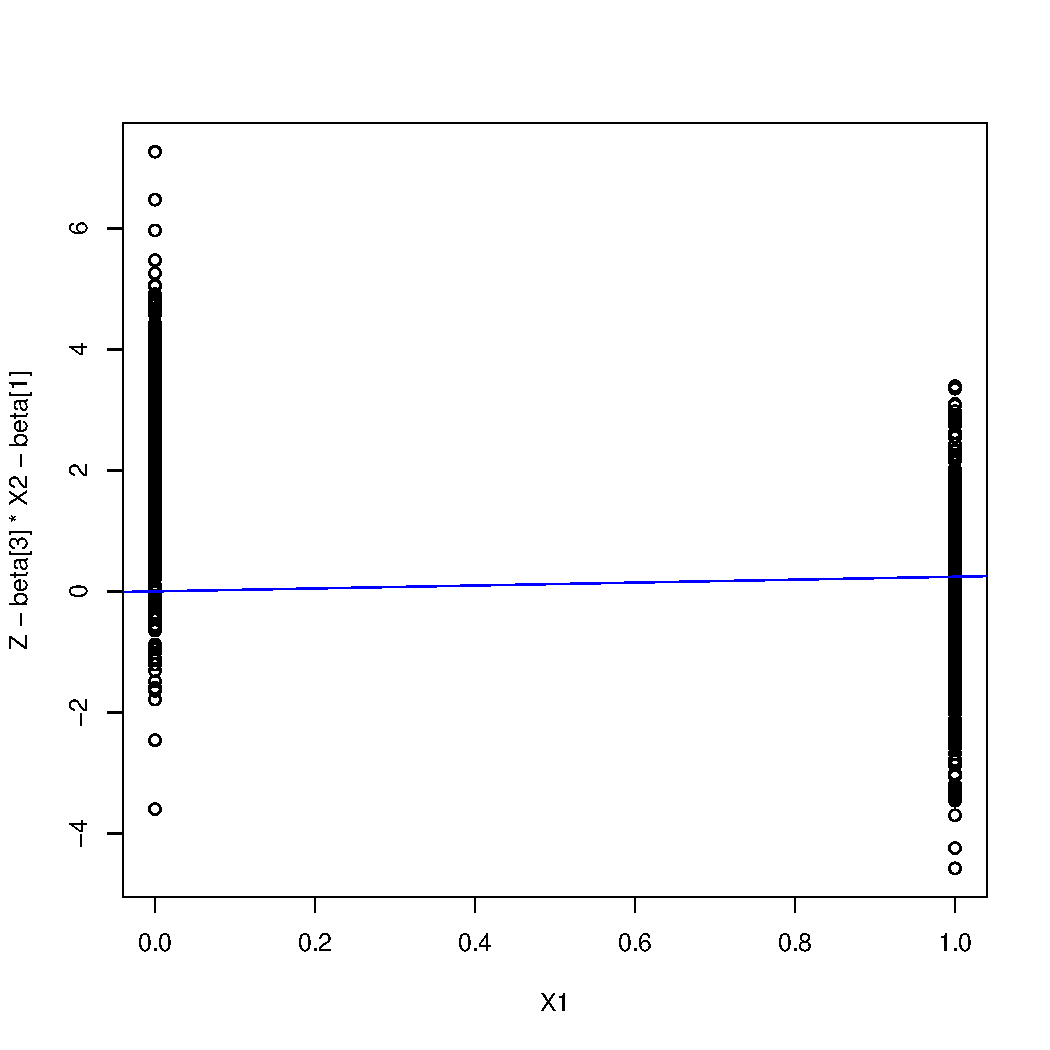
\includegraphics[scale=0.5]{p2x1.pdf}
\caption{$X_1$ and $Z$ with Regression Lines}
\label{p2x1}
\end{center}
\end{figure}

\begin{figure}[h!]
\begin{center}
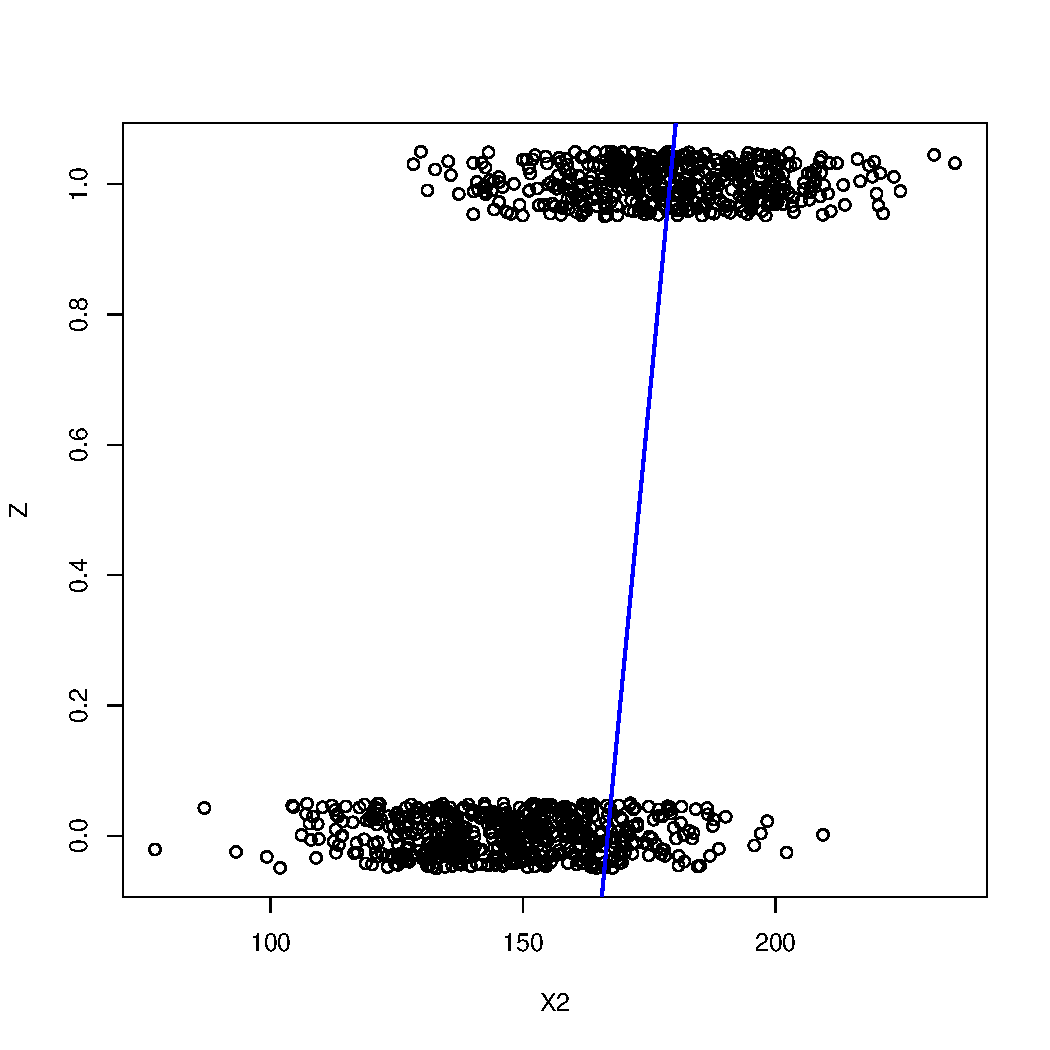
\includegraphics[scale=0.5]{p2x2.pdf}
\caption{$X_2$ and $Z$ with Regression Lines}
\label{p2x2}
\end{center}
\end{figure}

\paragraph{H} The correlation between the features $X_1$ and $X_2$ is high (0.63). This causes our estimates of $\beta$ to be biased, since it is difficult to isolate the impact of each feature. 

\paragraph{I} A model with only $X_2$ would do almost as well as the model with both features. This is due to the correlation between the two features and the relatively minimal impact of $X_1$ on the predicted $Z$ values, as shown in Figure \ref{p2x1}. As Figure \ref{p2x2} shows, risk for $Z$ increases noticeably when $X_2>160$, so this should be an important component of the researchers' decision rule. 

\end{answer}




\end{document}
